% ---------------------------------------------------------------------------
% Conference draft (3 pages) - proof of concept
%   "Reaching the Cramer-Rao Bound in Multi-Channel Transient Localisation"
%
% TODO before submission:
%   * authors / affiliations
%   * replace placeholder figures with the full-run versions
%     (results_crb_full_pairs/figs_estimators/*.png)
%   * verify the bibliography entries
% ---------------------------------------------------------------------------
\documentclass[10pt]{article}
\usepackage[a4paper,margin=0.85in]{geometry}
\usepackage{amsmath,amssymb}
\usepackage{graphicx}
\usepackage{booktabs}
\usepackage{xcolor}
\usepackage{tikz}
\usetikzlibrary{arrows.meta,positioning,calc,shapes.geometric}
\usepackage[hidelinks]{hyperref}
\usepackage{caption}
\captionsetup{font=small,labelfont=bf}
\setlength{\parskip}{3pt}
\setlength{\parindent}{0pt}
\graphicspath{{figures/}}

\newcommand{\SNR}{\mathrm{SNR}}
\newcommand{\SNReff}{\mathrm{SNR}_{\rm eff}}
\newcommand{\CRB}{\mathrm{CRB}}

\title{\vspace{-1.4em}\bfseries Reaching the Cram\'er--Rao Bound in Multi-Channel
Transient Localisation over WDM Links: Why Dispersion-Weighted Fusion Wins}
\author{\small Author names \quad \texttt{email@institution} \\ \small Affiliation}
\date{}

\begin{document}
\maketitle
\vspace{-2.0em}

\begin{abstract}
\noindent
A transient mechanical perturbation changes the state of polarisation (SOP)
along an optical link. Because of chromatic dispersion (CD), the perturbation
signature arrives at different times in different WDM channels, and the
inter-channel delay yields the perturbation distance. We derive the
\emph{two-sensor effective-SNR} Cram\'er--Rao bound (CRB) for this problem and
show, through an end-to-end PMD/CD simulation, that a \emph{dispersion-weighted}
fusion of channel pairs \emph{attains} the bound, whereas naive averaging does
not --- it can even be \emph{worse than the single best pair}. We give
signal-to-noise-ratio-free estimators, quantify the gain (up to
$\sim\!10^{2}$--$10^{3}\times$ lower RMSE than averaging and
$\sim\!10^{4}\times$ versus the worst pair), and report the scaling laws in
SNR, perturbation bandwidth, channel count and fibre count. The result is a
rigorous performance limit together with a simple design rule.
\end{abstract}

\section{Introduction}
\label{sec:intro}
Distributed optical sensing localises mechanical perturbations (vibration,
strain, acoustic transients) along a fibre and underpins applications from
infrastructure monitoring to intrusion detection~\cite{taylor1993das,he2022das}.
When the link carries a WDM comb, a single transient imprints a
\emph{wavelength-dependent} time delay: chromatic dispersion (CD) makes the
signature arrive earlier in some channels than in others. The delay between two
channels is proportional to the travelled distance, so estimating inter-channel
delays and inverting the CD integral gives a direct range measurement
\cite{sadler2003survey}. Using $\sim\!10$ WDM channels means hundreds of channel
pairs are available, which suggests fusing them for accuracy.

\smallskip
\noindent\textbf{This paper.} We make three points, at proof-of-concept level.
\emph{(i)}~We derive the CRB for CD-based transient localisation using the
two-sensor \emph{effective SNR}, and validate it against Monte Carlo.
\emph{(ii)}~We show a counter-intuitive result: naive \emph{equal-weight}
averaging across channel pairs is \emph{beaten by a single, well-chosen pair},
because low-separation pairs have huge variance. Only \emph{dispersion-weighted}
fusion approaches the CRB. \emph{(iii)}~We provide SNR-free estimators and the
scaling laws that make this a practical design rule.

\section{System Model and Cram\'er--Rao Bound}
\label{sec:model}
\textbf{Signal.} A fixed input SOP propagates through a fibre with
polarisation-mode dispersion (PMD, random wave-plate model) and CD. A transient
of bandwidth $B$ modulates the local birefringence over a short section at
distance $Z$. The received per-channel signal is the transmitted SOP, which we
represent by its 2-D Stokes projection $(S_1,S_2)$ after rotating the centroid
to the north pole. With channels at wavelengths $\lambda_i,\lambda_j$ the CD
delay is
\begin{equation}
\tau_{ij} = Z\,D_{ij},\qquad
D_{ij}=\int_{\lambda_j}^{\lambda_i}\! D(\lambda)\,d\lambda,\quad
D(\lambda)=D_0+S_0(\lambda-\lambda_0),
\label{eq:cd}
\end{equation}
so a pair-distance estimate is $\hat{Z}_{ij}=\hat{\tau}_{ij}/D_{ij}$.

\smallskip
\noindent\textbf{Energy SNR and bandwidth.} For a discrete signal $x[n]$ with
per-sample noise variance $\sigma^2$, the \emph{energy} SNR is
$\SNR=E/N_0=\sum_n x[n]^2/\sigma^2$, and the mean-square bandwidth is
\begin{equation}
\beta^2=\frac{\sum_k (2\pi f_k)^2|X_k|^2}{\sum_k |X_k|^2}.
\label{eq:beta}
\end{equation}
For two noisy observations of a common signal the delay information is set by
the \emph{effective} SNR,
\begin{equation}
\SNReff(f)=\frac{\rho_1\rho_2}{1+\rho_1+\rho_2},\qquad
\rho_i(f)=\frac{S(f)}{N_i(f)},
\label{eq:effsnr}
\end{equation}
which for equal sensors reduces to $\rho^2/(1+2\rho)$. The Fisher information
and CRB follow as
\begin{equation}
J_{ij}=\sum_k \omega_k^2\,\SNReff(f_k),\qquad
\CRB(\tau_{ij})=1/J_{ij},\qquad
\sigma_{Z,ij}=\frac{\sqrt{\CRB(\tau_{ij})}}{D_{ij}} .
\label{eq:crb}
\end{equation}
At high SNR $\SNReff\!\to\!\rho/2$ and $\CRB=1/(\SNR\beta^2)$: \emph{bandwidth
and SNR are the fundamental limits}. Equation~\eqref{eq:crb} is the reference
used throughout.

\begin{figure}[t]
\centering
\begin{tikzpicture}[font=\small,>=Latex,node distance=5mm]
\node[draw,rounded corners,minimum height=6mm,minimum width=11mm] (tx){TX};
\node[draw,rounded corners,minimum height=6mm,minimum width=34mm,right=8mm of tx] (link){fibre link \ (PMD + CD)};
\node[right=8mm of link,star,star points=6,star point height=2.2mm,draw,fill=red!60,inner sep=0pt,minimum size=4mm] (ev){};
\node[below=1mm of ev,text=red!70!black] (evl){perturbation at $Z$};
\node[draw,rounded corners,minimum height=6mm,minimum width=12mm,right=8mm of ev] (rx){WDM};
\node[draw,rounded corners,minimum height=6mm,below=6mm of rx,minimum width=12mm] (dsp){fusion};
\draw[->] (tx)--(link); \draw[->] (link)--(ev); \draw[->] (ev)--(rx);
\draw[->] (rx)--(dsp);
\node[right=1mm of rx,align=left,font=\footnotesize] {$\lambda_1\!:\!\tau_1$\\$\lambda_2\!:\!\tau_2$\\$\vdots$};
\end{tikzpicture}
\caption{Concept. A single transient imprints wavelength-dependent delays
$\tau_i\propto Z\!\int\! D\,d\lambda$; multi-channel fusion recovers $Z$.}
\label{fig:concept}
\end{figure}

\section{Multi-Channel Fusion Estimators}
\label{sec:fusion}
Given one estimate $\hat{Z}_{ij}$ per channel pair, the distance is a weighted
mean $\hat{Z}=\sum_{ij} w_{ij}\hat{Z}_{ij}/\sum_{ij} w_{ij}$. We compare four
\emph{SNR-free} rules (only $D_{ij}$ is needed):
\begin{itemize}\itemsep1pt
\item \textbf{Single pair}: one pair only (best = largest $D$, or worst = smallest $D$).
\item \textbf{Average}: $w_{ij}=1$ (naive).
\item \textbf{Dispersion-weighted}: $w_{ij}=D_{ij}^2$. This is the
minimum-variance (inverse-variance) weight because
$\sigma_{Z,ij}\propto 1/D_{ij}$ when the per-pair delay CRB is common.
\item \textbf{Robust}: $w_{ij}=D_{ij}^2\,\psi(r_{ij})$, with a Tukey-bisquare
$\psi(r)=(1-(r/(c\,s))^2)^2$ on residuals $r_{ij}=|\hat Z_{ij}-\mathrm{med}(\hat Z)|$,
scale $s=\mathrm{IQR}$ --- it tames threshold-region outliers.
\end{itemize}
\emph{Caveat.} Pair estimates share channels and are therefore correlated; a
strict bound requires the full covariance (a structured GLS combination). We use
the effective-SNR CRB as a tight practical reference and discuss the
correlation penalty in the text.

\section{Results}
\label{sec:results}
\noindent\textbf{Setup.} We simulate $10$ independent PMD fibres, a C+L WDM comb
(241 channels, 50~GHz), perturbation bandwidth $B\in[200\,\mathrm{Hz},2\,\mathrm{MHz}]$,
energy SNR $\in[15,100]\,\mathrm{dB}$, $100$ noise realisations, and channel
subsets of size $4$--$12$ (extremes first). Delays are estimated by parabolic
interpolation of the 2-D cross-correlation.

\begin{figure}[t]
\centering
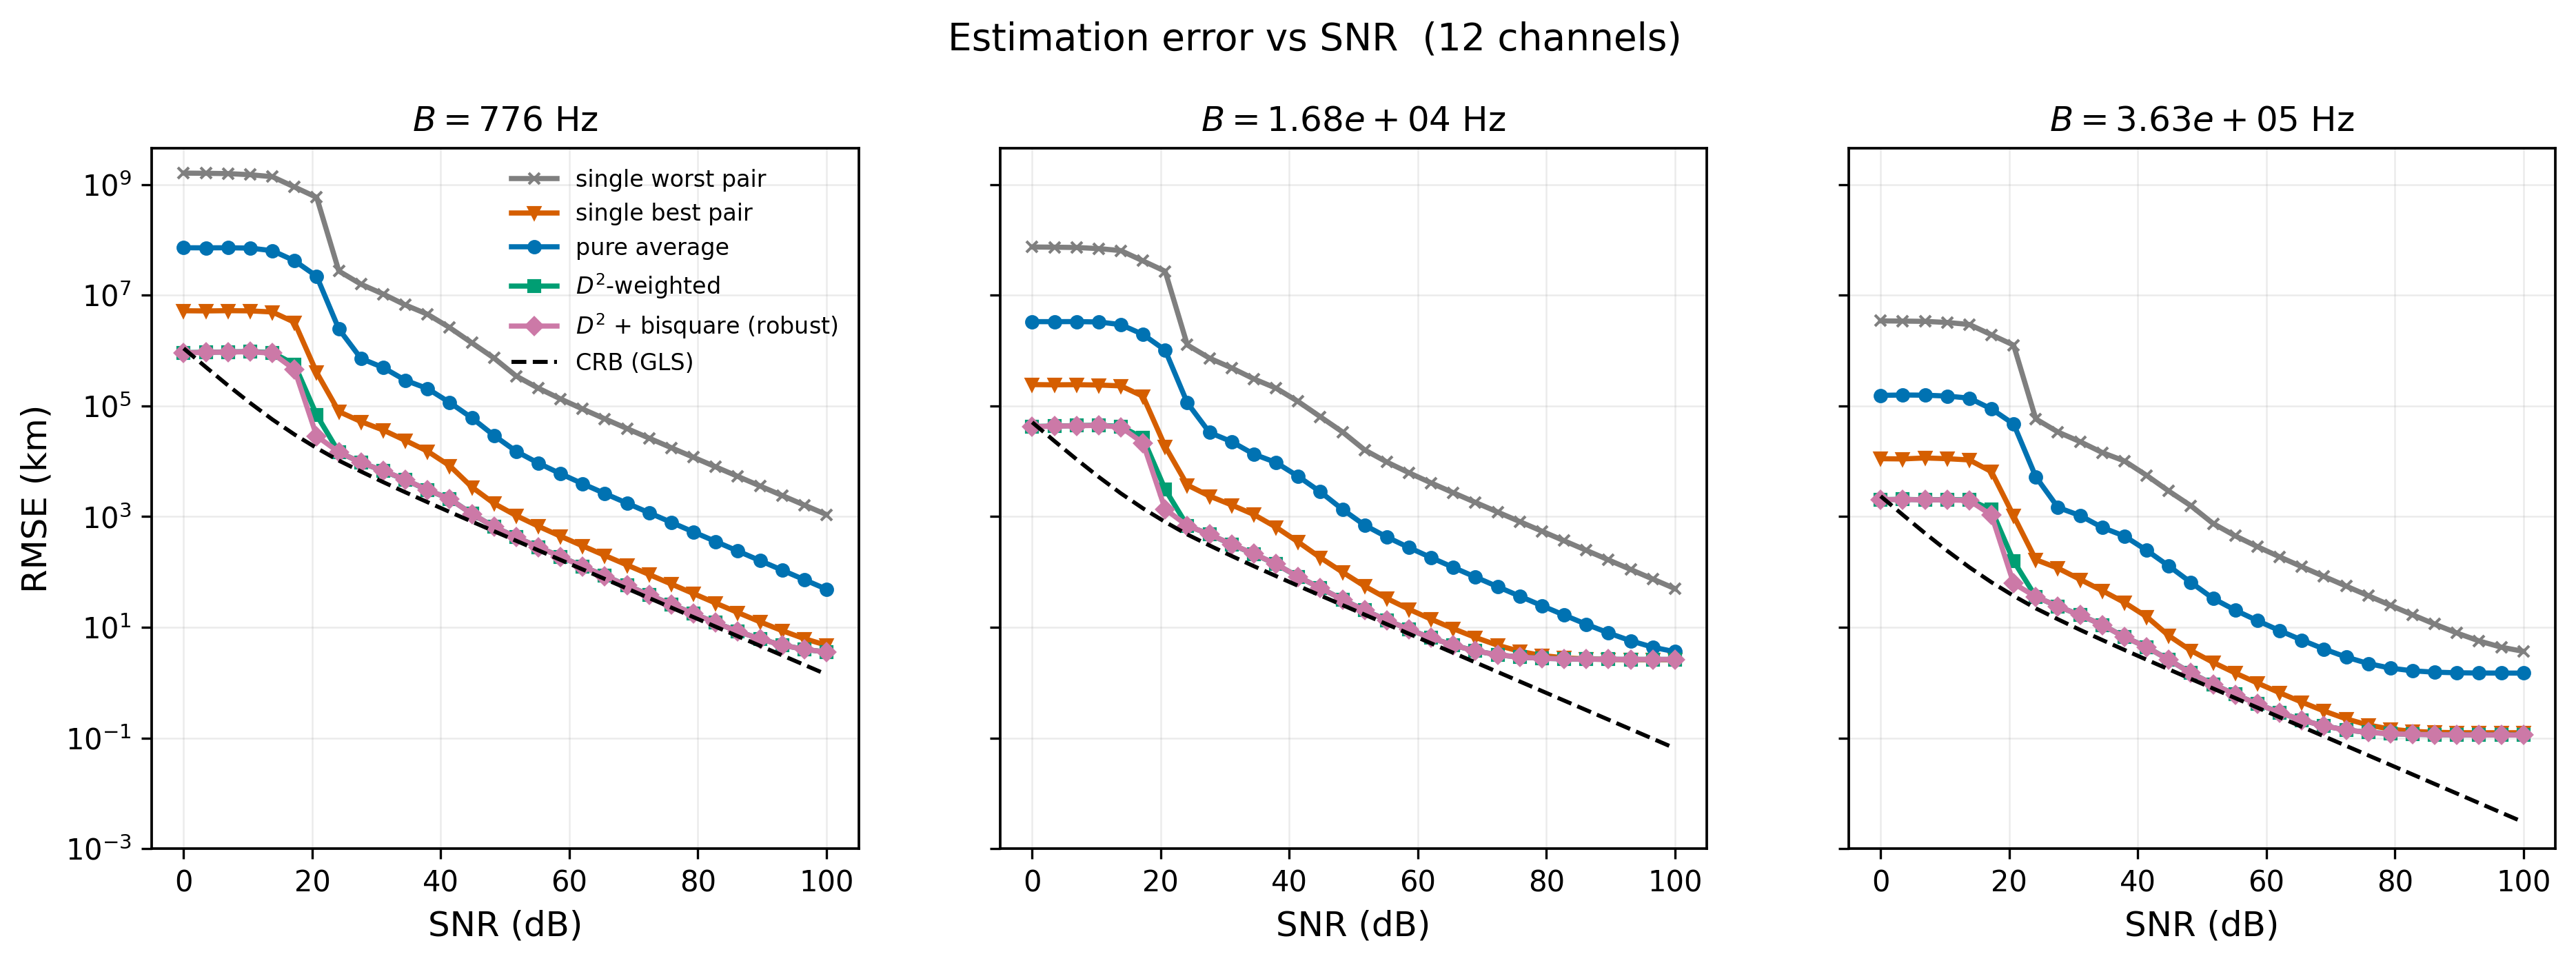
\includegraphics[width=\linewidth]{F1_rmse_vs_snr.png}
\caption{RMSE vs SNR at three bandwidths ($12$ channels). The ranking is
striking: \emph{worst pair} $\gg$ \emph{pure average} $>$ \emph{best pair}
$>$ dispersion-weighted $\approx$ robust $\approx$ CRB. Equal-weight averaging
is \emph{worse than one well-chosen pair}; dispersion weighting attains the
bound.}
\label{fig:money}
\end{figure}

\noindent\textbf{Fusion reaches the CRB; averaging does not
(Fig.~\ref{fig:money}).} At high SNR, dispersion-weighted fusion and the robust
variant sit on the CRB (RMSE/CRB $\approx 1.0$--$1.1$), while the single best
pair remains $1$--$10\times$ and pure averaging
$10$--$10^{3}\times$ above it. The worst pair is catastrophically bad, up to
$\sim\!10^{4}\times$ the fused estimate. The physical reason is
Eq.~\eqref{eq:crb}: since $\sigma_{Z,ij}\propto 1/D_{ij}$, low-separation pairs
carry almost no information, yet equal weighting lets them dominate.

\begin{figure}[t]
\centering
\begin{minipage}{0.49\linewidth}\centering
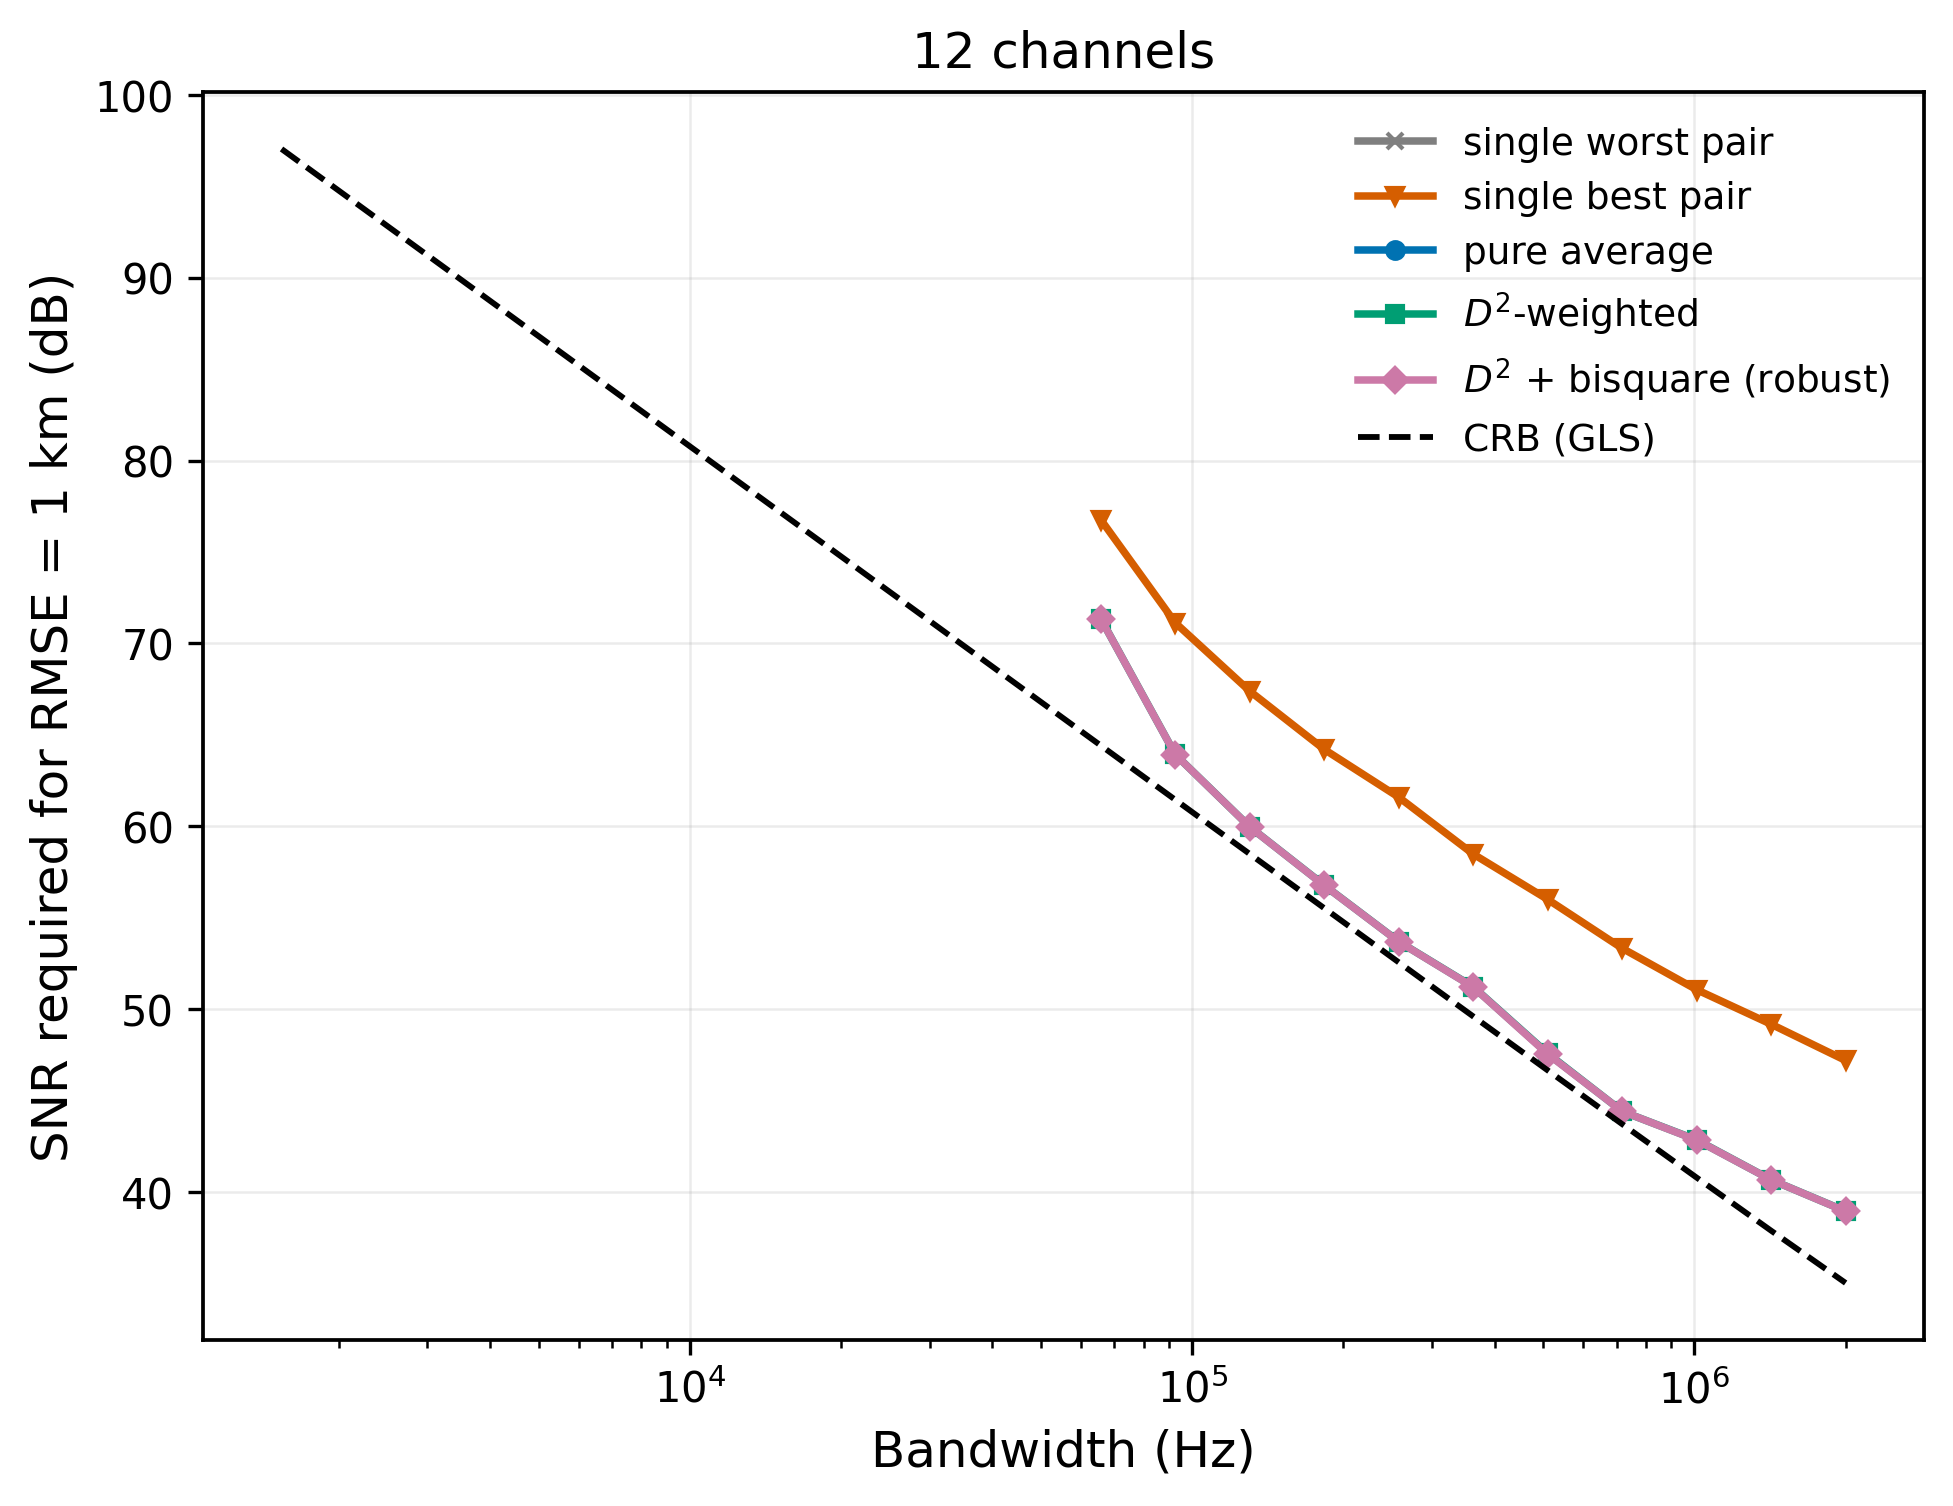
\includegraphics[width=\linewidth]{F3_isoprecision.png}
\end{minipage}\hfill
\begin{minipage}{0.49\linewidth}\centering
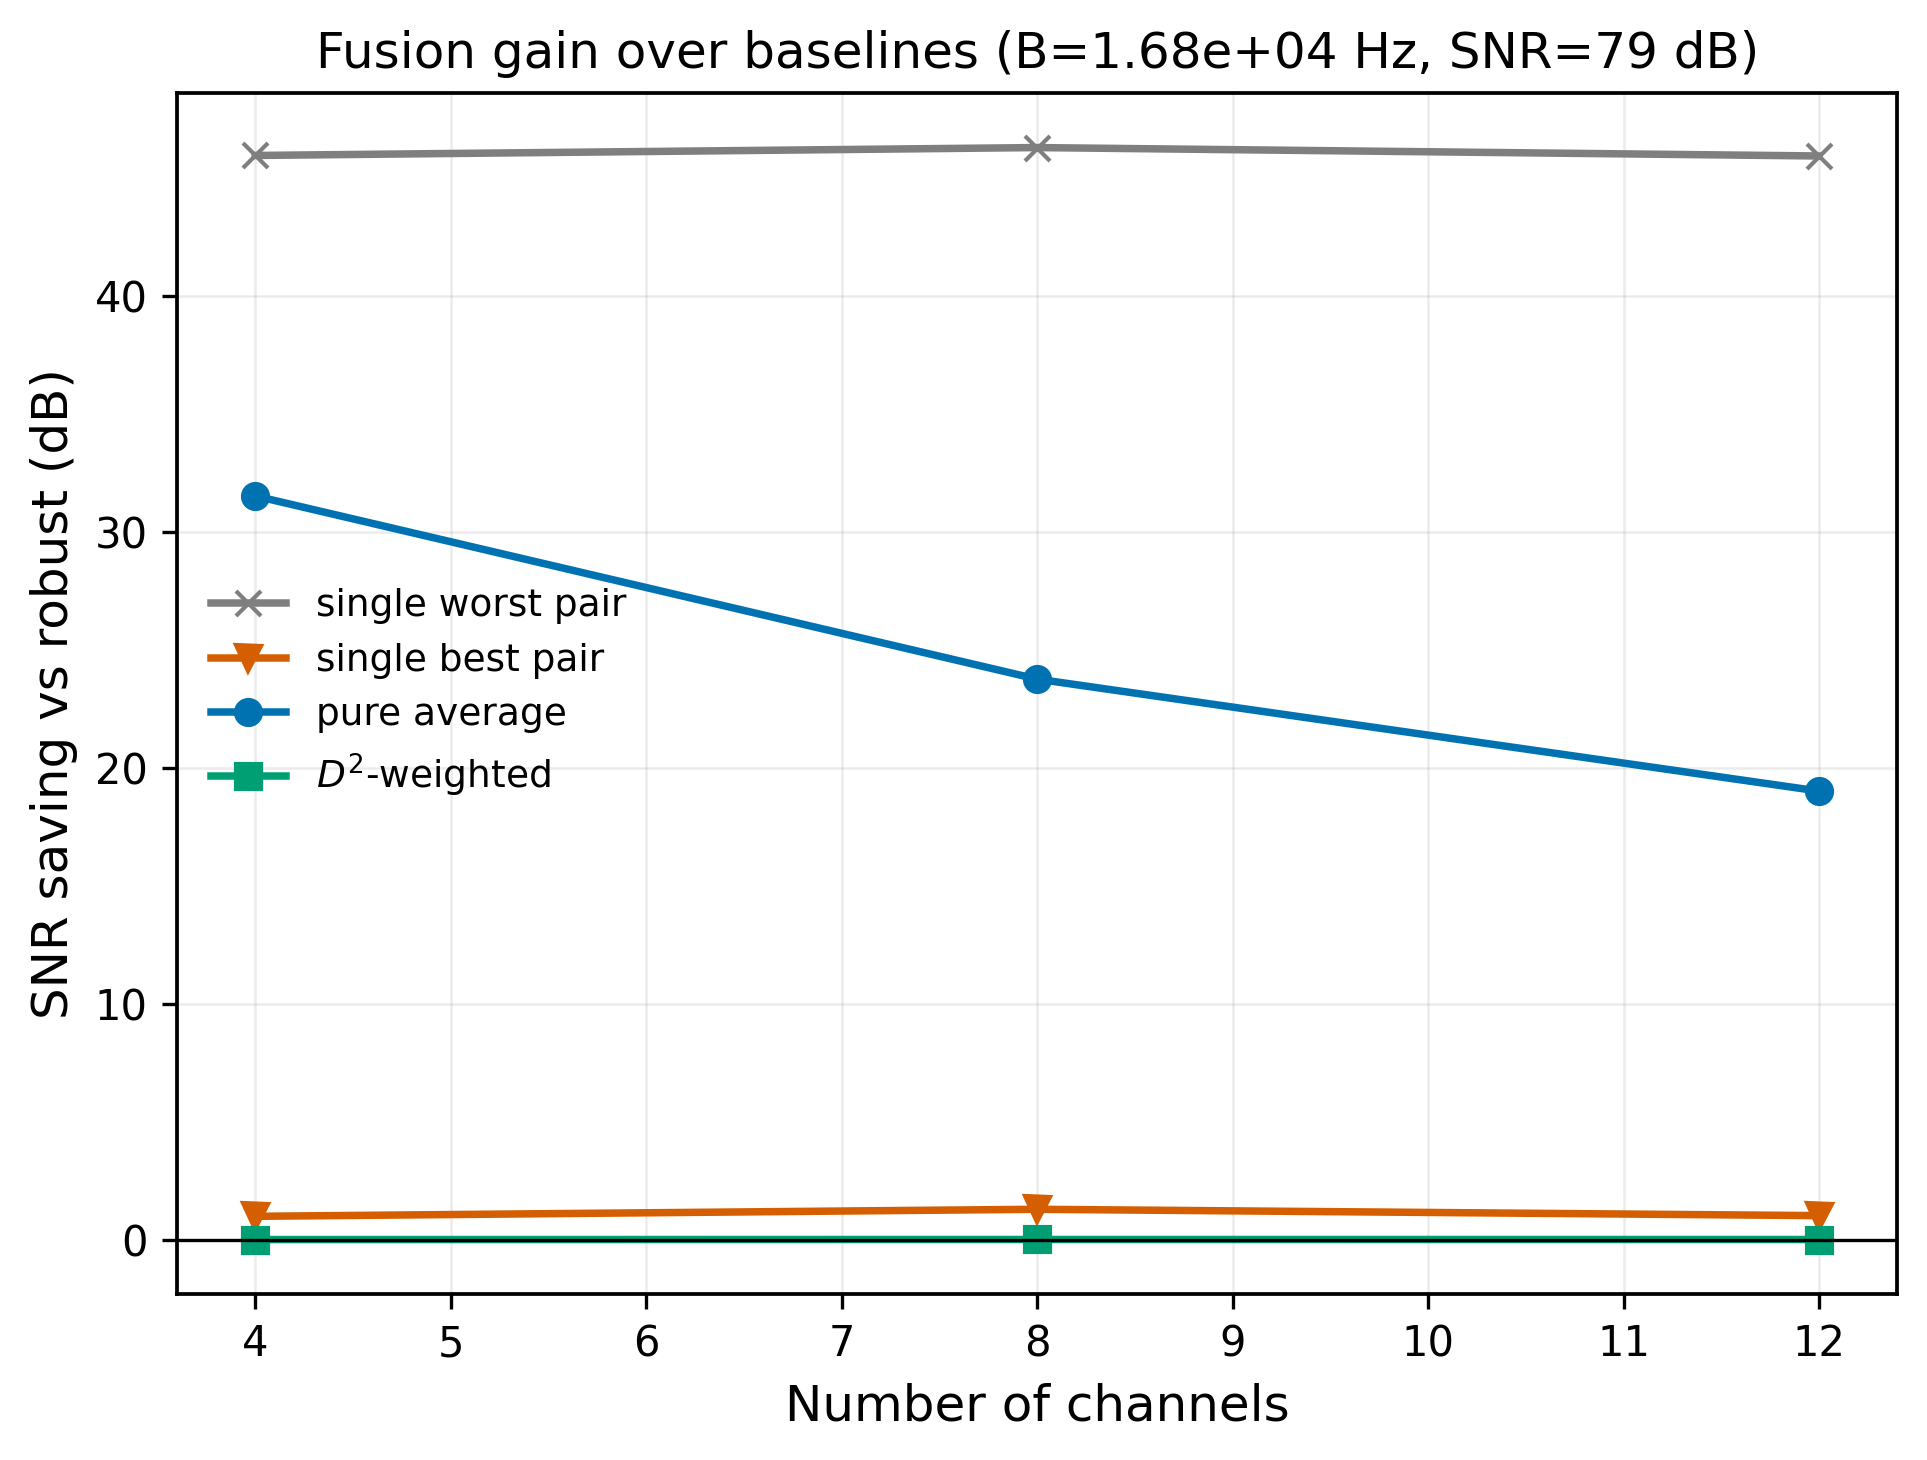
\includegraphics[width=\linewidth]{F4_db_gain_vs_channels.png}
\end{minipage}
\caption{Design curves. Left: SNR required for RMSE $=1$~km vs perturbation
bandwidth (each curve an estimator; dashed = CRB). Right: SNR saving of
dispersion-weighted fusion over the baselines versus number of channels --- the
fusion gain \emph{grows} with the channel count.}
\label{fig:scaling}
\end{figure}

\noindent\textbf{Scaling laws (Fig.~\ref{fig:scaling}).} (i)~At high SNR the
RMSE scales as $1/(\sqrt{\SNR}\,B)$, recovering the CRB law
Eq.~\eqref{eq:crb}: the perturbation \emph{bandwidth is as fundamental as SNR}.
(ii)~Adding channels increases the fused information through $\sum D_{ij}^2$;
the SNR saving over a single pair grows with channel count (Fig.~\ref{fig:scaling},
right). (iii)~Averaging $N$ independent fibres reduces the RMSE as
$1/\sqrt{N}$, independently of the fusion rule. (iv)~The robust rule only
diverges from the CRB in the threshold region, where it lowers both RMSE and
heavy-tail bias.

\section{Conclusion}
\label{sec:conclusion}
We derived and validated the effective-SNR CRB for CD-based transient
localisation and showed that \emph{dispersion-aware} multi-channel fusion
reaches it, while naive averaging can be worse than a single optimised pair.
Because the winning estimator needs no SNR knowledge, it is directly
deployable; and because the bound depends on $\sqrt{\SNR}\cdot B$, it also tells
us that slow perturbations are the hard case. Future work: experimental
validation and a covariance-aware (GLS) fusion.

\begin{thebibliography}{9}\small
\bibitem{taylor1993das} H.~F. Taylor and C.~E. Lee, ``Apparatus and method for
fiber optic intrusion sensing,'' U.S. Patent 5,194,847, 1993.
\bibitem{he2022das} Z.~He and Q.~Liu, ``Optical fiber distributed acoustic
sensing: a review,'' \emph{Photonics}, vol.~9, no.~4, 2022.
\bibitem{sadler2003survey} B.~M. Sadler and R.~J. Kozick, ``A survey of time
delay estimation performance bounds,'' in \emph{IEEE Workshop on Statistical
Signal Processing}, 2003.
\bibitem{weiss1983} A.~J. Weiss and E.~Weinstein, ``Fundamental limitations in
passive time-delay estimation---Part I,'' \emph{IEEE Trans. Acoust., Speech,
Signal Process.}, vol.~31, no.~2, 1983.
\bibitem{ziv1969} J.~Ziv and M.~Zakai, ``Some lower bounds on signal parameter
estimation,'' \emph{IEEE Trans. Inf. Theory}, vol.~15, no.~3, 1969.
\bibitem{gisin1992} N.~Gisin and J.~P. Pellaux, ``Polarization mode dispersion:
time versus frequency domains,'' \emph{Opt. Commun.}, vol.~89, 1992.
\end{thebibliography}

\end{document}
